
\subsection{Extended Kalman Filter (EKF)}
The Kalman filter (KF) provides a more sophisticated approach, estimating the true state of the system by minimizing the mean of the squared error. It involves prediction and update steps. However,  assumes that both the process and measurement models are linear. However, many real-world systems, such as robotic motion and sensor fusion, exhibit inherent nonlinearities. When linearization is not feasible, the standard KF becomes inaccurate. 

To address this limitation, the Extended Kalman Filter (EKF) extends the KF to nonlinear systems by employing a first-order Taylor series expansion. This method approximates the nonlinear system dynamics and measurement models with locally linearized representations, allowing the filter to be applied in scenarios where exact linearization is not feasible.

The EKF is an extension of the Kalman Filter for nonlinear systems, utilizing first-order Taylor series expansion to linearize process and measurement models. EKF maintains a Gaussian belief over the state, updating it through a prediction-correction cycle. The Jacobian matrices of the system dynamics and measurement functions are used to approximate state transitions and measurement updates. Its advantages include handling nonlinearities, fusing multi-sensor data, and improving estimation accuracy in noisy environments. 

\subsubsection{General State Equation}
For non-linear system, with Stochastic disturbances:
\begin{equation}
\begin{aligned}
	\dot{\underline{x}}(t) &= f\left( \underline{x}(t), \underline{u}(t) \right) + \underline{d}(t) \\
	\underline{y}(t) &= h\left( \underline{x}(t) \right) + \underline{n}(t)
\end{aligned}
\end{equation}
where,
\begin{itemize}
	\item $ \dot{\underline{x}}(t) $: This represents the time derivative of the state vector $ \underline{x}(t) $, indicating how the state evolves over time.
	\item $ f $: This is a nonlinear function that describes the system dynamics, taking the current state $ \underline{x}(t) $ and the control input $ \underline{u}(t) $ as arguments. It captures how the state changes based on the current state and control inputs.
	\item $ \underline{d}(t) $: This term represents stochastic disturbances (or process noise) affecting the state dynamics, typically modeled as a zero-mean Gaussian noise.
	\item $ y(t) $: This is the measurement vector at time $ t $, representing the observed outputs of the system. It is the data collected from sensors or measurement devices.
	\item $ h $: This is a nonlinear measurement function that maps the true state vector $ \underline{x}(t) $ to the measurement space. It describes how the state influences the measurements. The function $ h $ can be complex and may involve various transformations of the state variables.
	\item $ n(t) $: This term represents measurement noise, which is also typically modeled as zero-mean Gaussian noise. It accounts for inaccuracies in the measurements due to sensor errors, environmental conditions, or other random factors that can affect the observed data.
\end{itemize}

\subsubsection{State Estimation}
For a non-linear system the state form is as follows,
\begin{equation}
\begin{aligned}
	\dot{\hat{\underline{x}}}(t) &= f\left( \underline{\hat{x}}(t), \underline{u}(t) \right) + \underline{K}\left( y(t) - \hat{y}(t) \right) \\
	\hat{y}(t) &= h\left( \underline{\hat{x}}(t) \right)  \label{eq:eq}
\end{aligned}
\end{equation}
The Kalman gain $\underline{K}$ is computed to optimally balance estimation uncertainty and measurement noise. To achieve this, the system is first linearized around the current state estimate by computing the Jacobians of the process and measurement models. To linearize the system around the current state estimate, the Jacobian matrices, which represent the first-order partial derivatives of the nonlinear functions, are computed as follows:
\begin{equation}
\underline{A}(t) = \frac{\mathrm{d}f}{\mathrm{d}\underline{x}} \bigg|_{\underline{\hat{x}}(t), \underline{u}(t)} \quad \text{and} \quad
\underline{C}(t) = \frac{\mathrm{d}h}{\mathrm{d}\underline{x}} \bigg|_{\underline{\hat{x}}(t)}  \label{eq:eq}
\end{equation}
where $\underline{A}(t)$ represents the partial derivatives of the state dynamics function $f$ and $\underline{C}(t)$ represents the partial derivatives of the measurement function $h$.
\begin{figure}[h]
	\centering
	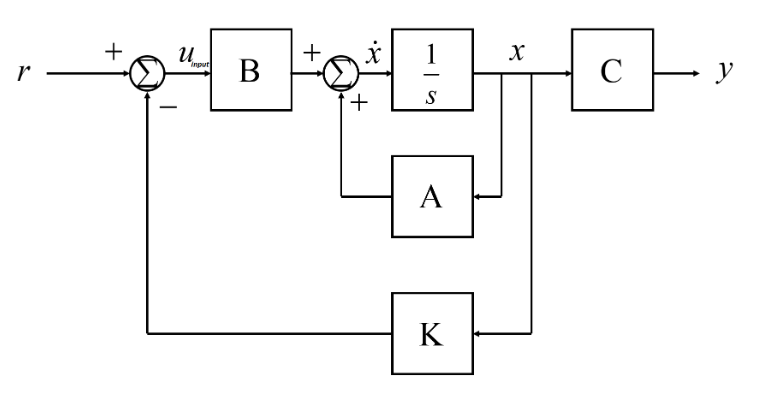
\includegraphics[height=5cm]{assets/block_representation_kalman_filter.png}
	\caption{Block representation of state space system showing the system matrices $A$, $B$ and $C$ as well as the gain matrix $K$.}
	\label{fig:block_representation_kalman_filter}
\end{figure}
\subsubsection{Covraince Matrix}
The evolution of the state estimation covariance matrix follows the continuous-time Riccati equation, given by:
\begin{equation}
\dot{P}(t) = \underline{A}(t) P(t) + P(t) \underline{A}^T(t) + Q - P(t) \underline{C}^T(t) R^{-1} \underline{C}(t) P(t)  \label{eq:eq}
\end{equation}
Where, 
\begin{itemize}
	\item $\dot{P}(t)$: his represents the time derivative of the covariance matrix $\dot{P}(t)$, which quantifies the uncertainty in the state estimate over time.
	\item $\underline{A}(t)$: This is the state transition matrix, which describes how the state evolves from one time step to the next.
	\item $Q$: This is the process noise covariance matrix, representing the uncertainty in the process model.
	\item $\underline{C}(t)$: This is the measurement matrix, which relates the state to the measurements.
	\item $R$: This is the measurement noise covariance matrix, representing the uncertainty in the measurements.
\end{itemize}
The Kalman filter is initialized with an initial covariance matrix:
\begin{equation}
	P(0) = \mathbf{E}(\Delta\underline{x}(0) \Delta\underline{x}^T(0))  \label{eq:eq}
\end{equation}
The optimal Kalman gain, balancing estimation uncertainty and measurement noise, is given by:

\begin{equation} \underline{K}(t) = P(t) \underline{C}^T R^{-1} \end{equation}
The time-discrete Kalman filter state update equations are:
\begin{equation}
	\begin{aligned}
		\underline{x}_{k} &= \underline{A} \underline{x}_{k-1} + \underline{B} \underline{u}_{k} + \underline{d}_{k-1} \\
		\underline{y}_{k} &= \underline{C} \underline{x}_{k} + \underline{n}_{k}  \label{eq:eq}
	\end{aligned}
\end{equation}
where $\underline{x}_k$ is the state vector, $\underline{B}$ the control input matrix, and $\underline{y}_k$ the measurement vector. The discrete state-space representation is:
\begin{equation}
	\begin{aligned}
		\underline{\dot{x}}(t) = \underline{A}.\underline{x}(t) + \underline{B}.\underline{u}(t) \\
		\underline{y}(t) = \underline{C}.\underline{x}(t) + \underline{D}.\underline{u}(t)  \label{eq:eq}
	\end{aligned}
\end{equation}
The state covariance matrix is:
\begin{equation}
	\mathbf{P}_k = \begin{bmatrix} P_{00} & P_{01} \\ P_{10} & P_{11} \end{bmatrix}  \label{eq:eq}
\end{equation}
where $P_{00}$ represents uncertainty in the angle estimate and $P_{11}$ in gyroscope bias. The Kalman gain is computed as:
\begin{equation}
	\begin{aligned}
		\underline{K}_{k} &= \underline{P}_{k}^- \ \underline{C}^T ( \underline{C} \ \underline{P}_{k}^-\ \underline{C}^T  +\underline{R})^{-1} \\ \\
		\mathbf{K}_k &= \begin{bmatrix} \frac{ P_{00} }{ P_{00}  
				+ R_{angle}} \\ \frac{ P_{10} }{ P_{00}  
				+ R_{angle}} \end{bmatrix}
	\end{aligned}  \label{eq:eq}
\end{equation}
Following the prediction step, the measurement update step refines the state estimate using the Kalman gain, which is derived to minimize the posterior estimation error covariance (see Appendix \ref{appendix:B} for detailed calculations):
\begin{equation}
	\begin{aligned}
		\underline{P}_{k} &= \ (\underline{I} - \underline{K}_{k} \ \underline{C}) \ \underline{P}_{k}^- \label{eq:eq}
	\end{aligned}
\end{equation}


\subsection{Software Implementation of EKF}
For the implementation of the Extended Kalman Filter (EKF), we utilized the Kalman filter library developed by Kristian Lauszus~\cite{github_kalman_filter}. This library was modified in accordance with the GNU General Public License to meet the specific requirements of our project.
\begin{lstlisting}[style=cppstyle2]
#include <Arduino.h>

class KalmanFilter {
 private:
  float m_dt, m_Q_angle, m_Q_gyro, m_R_angle, m_C_0;
  float q_bias = 0, angle_err = 0;
  float P[2][2] = {{1, 0}, {0, 1}}; // Covariance matrix
  float K_0 = 0, K_1 = 0;

 public:
  float angle = 0;

KalmanFilter(float dt, float Q_angle, float Q_gyro, float R_angle, float C_0)
: m_dt(dt), m_Q_angle(Q_angle), m_Q_gyro(Q_gyro), m_R_angle(R_angle), m_C_0(C_0) {}

float getAngle(float measured_angle, float measured_gyro) {
	// Predict
	angle += (measured_gyro - q_bias) * m_dt;
	angle_err = measured_angle - angle;
	
	// Update covariance matrix
	P[0][0] += m_Q_angle - P[0][1] - P[1][0];
	P[0][1] -= P[1][1];
	P[1][0] -= P[1][1];
	P[1][1] += m_Q_gyro;
	
	// Compute Kalman gain
	float E = m_R_angle + m_C_0 * P[0][0];
	K_0 = (m_C_0 * P[0][0]) / E;
	K_1 = (m_C_0 * P[1][0]) / E;
	
	// Update state
	angle += K_0 * angle_err;
	q_bias += K_1 * angle_err;
	
	// Update covariance matrix
	float C0_P00 = m_C_0 * P[0][0];
	P[0][0] -= K_0 * C0_P00;
	P[0][1] -= K_0 * P[0][1];
	P[1][0] -= K_1 * P[0][0];
	P[1][1] -= K_1 * P[0][1];
	
		return angle;
	}
};
\end{lstlisting}